
\chapter{Elaborazione dei segnali}

Chi lavora con i segnali vede il segnale come un oggetto adimensionale,
trattando il concetto di \textit{potenza} ed \textit{energia} di un segnale
senza vedere effettivamente il senso e la grandezza fisica del segnale.
Esistono i segnali di tipo \textbf{deterministico} e segnali di tipo
\textbf{aleatorio}.
Se il segnale è di natura deterministica sono in grado di determinare
l'espressione del segnale, se invece è di natura aleatoria non posso
determinare in forma chiusa il suo andamento, data appunto la sua natura
stocastica, aleatoria.

Un segnale è una grandezza fisica o misurabile che evolve nel tempo, il
segnalamento sta nelle caratteristiche dell'evoluzione temporale.
Nel caso limite il segnale può essere banale ossia costante nel tempo.

Un segnale è detto di energia ed è dotato di energia se la grandezza
\begin{equation}
 \varepsilon_x = \int_{-\infty}^{+\infty} |x(t)|^2 dt < +\infty
\end{equation}
è finita, tutti i segnali transitori che decadono in un certo intervallo di
tempo sono segnali di energia.

La potenza di un segnale è definita come
\begin{equation}
 P_x = \lim_{T\to+\infty} \left(\frac{1}{T}\int_{-T/2}^{+T/2} |x(t)|^2
dt\right) < +\infty
\label{eq:potenza_segnale}
\end{equation}

Il segnale sinusoidale ad esempio non è un segnale di energia ma è un segnale
di potenza, se si valuta il valor medio su un intervallo pari ad un periodo o
multiplo di periodo, si può determinare la potenza del segnale.

In base alle definizioni l'energia si esprime ad esempio in $V^2/s$ mentre la
potenza rimarrebbe $V^2$, anche se non ci sarebbe alcuna correlazione fisica con
la potenza elettrica. Ci sarebbe corrispondenza tra potenza del segnale e
potenza elettrica se il segnale fosse proprio $v(t)\cdot i(t)$ o nel caso
semplice $|v(t)|^2/R$.

\section{I segnali periodici}
Tipicamente in ingegneria elettrica i segnali analizzati sono periodici,
possono essere più o meno distorti ma sempre riconducibili a serie di segnali
periodici.
La classe di segnali periodici si identifica come la classe di segnali che
soddisfa il vincolo
$$
x(t+kT_0) = x(t) \forall k \in \mathrm{Z}
$$
dove $T_0$ è proprio il periodo del segnale.

Se un segnale è semplice si può esprimere con una semplice funzione
sinusoidale, oppure esistono segnali di forma canonica come i segnali
triangolari o ad onda quadra, in alternativa si può rappresentare un segnale
periodico con la sua serie di Fourier
\begin{equation}
 x(t) = A_0 + \sum_{k=1}^{\infty} A_k \cos \left( 2\pi f_0 t - \phi_k \right)
\end{equation}
con $f_0= \frac{1}{T_0}$ la frequenza fondamentale, per $k$ diverso da uno
invece si hanno altre frequenze chiamate componenti armoniche perché sono un
multiplo intero della frequenza fondamentale.
Il termine $A_0$ rappresenta la componente continua, se diversa da 0 il segnale
non è alternato.

Il termine sinusoidale si può scomporre con un termine in fase ed uno in
quadratura.

\begin{equation}\begin{aligned}
 \cos(\alpha-\beta) &= \cos\alpha\cos\beta+\sin\alpha\sin\beta \\
 x(t) &= A_0 + \sum_{k=1}^{\infty} \left[ A_k\cos\phi_k\cos(2\pi k f_0 t) +
A_k\sin\phi_k\sin(2\pi k f_0t) \right] \\
x(t) &= a_0 + \sum_{k=1}^{\infty}\left[a_k\cos(2\pi k f_0) + b_k\sin(2\pi k
f_0)\right]
\end{aligned}
 \end{equation}

I due termini sono dunque in quadratura tra loro
\begin{equation*}
\begin{aligned}
\left\{\begin{aligned}
a_k &= A_k\cos\phi_k\\
b_k &= A_k\sin\phi_k
\end{aligned}\right. \\
&\text{dunque}\\
A_k &= \sqrt{a_k^2 + b_k^2}\\ \left\{
\begin{aligned}
\phi_k &= \tan^{-1}\left(\frac{b_k}{a_k}\right) \quad a_k > 0 \\
 \phi_k &=\pi - \tan^{-1} \left(\frac{b_k}{a_k}\right) \quad a_k < 0
 \end{aligned}\right.
\end{aligned}
\end{equation*}

Si ricorda la seguente definizione della formula di Eulero
\begin{equation}
 e^{\pm jx} = \cos{x} \pm j\sin{x}
\end{equation}
con la scomposizione in serie si può esprimere la funzione esponenziale
con la seguente forma
\begin{equation*}
e^x = \sum_{n=0}^{\infty} \frac{x^n}{n!} = 1+x+\frac{x^2}{2}+ \dots
\end{equation*}

Se le serie hanno segno alternato, ossia sono serie oscillanti, allora si può
estrarre le rappresentazioni delle serie proprie di seno e coseno.

Utilizzando le formule di Eulero si riscrive la serie del segnale
\begin{equation*}\begin{aligned}
 x(t) &= a_0 + \sum_{k=1}^{+\infty} a_k \frac{e^{j2\pi kf_0t} + e^{-j2\pi
kf_0t}}{2} + b_k \frac{e^{j2\pi kf_0t}-e^{-j2\pi kf_0t}}{2j} \\
&=  a_0 + \sum_{k=1}^{+\infty}\left[\frac{a_k-jb_k}{2}e^{j2\pi k f_0 t} +
\frac{a_k+jb_k}{2} e^{-j2\pi kf_0 t} \right]
\end{aligned}\end{equation*}
 raggruppando i coefficienti si ottiene
 $$\begin{aligned}
 c_k &= \frac{a_k-jb_k}{2} \\
 c_k^* &= \frac{a_k+jb_k}{2}
 \end{aligned}$$
Il segnale in forma compatta diventa
 $$
 x(t) = \sum_{k=-\infty}^{+\infty} c_k e^{j2\pi k f_0 t}
 $$
Si è ottenuta un'espressione estremamente compatta.
Lavorando sulle precedenti espressioni si ricava
$$\begin{aligned}
|c_k| &= c_k\cdot c_k^* = \frac{A_k}{2}\\
\angle c_k &= \tan^{-1}_4\left(\frac{b_k}{a_k}\right)
\end{aligned}$$

Dato un segnale generico si può scomporre in serie ed ottenere i due
coefficienti con le seguenti formule:
$$\begin{aligned}
a_k &= \frac{2}{T_0} \int_{T_0} x(t)\cos(2\pi k f_0 t) dt\\
b_k &= \frac{2}{T_0} \int_{T_0} x(t)\sin(2\pi k f_0 t) dt
\end{aligned}$$

Viceversa per il calcolo di $c_k$ si ottiene
$$
c_k = \frac{1}{T_0}\int_{T_0} x(t) e^{-j2\pi k f_0 t}dt
$$
ciò che identifica il segnale diventa esclusivamente il valore dei coefficienti
$c_k$


Se si lavora in regime periodico distorto, grazie alla scomposizione armonica
si può studiare la potenza dissipata da ciascuna armonica, analizzando sempre
la rete con il PSE, pensando che questa sia sollecitata a tante sorgenti
ciascuna sollecitata a frequenze diverse, l'ampiezza $\frac{A_k}{\sqrt2}$ sarà
il valor efficace della singola armonica mentre la potenza per l'armonica
k-esima sarà $\frac{A_k^2}{2}$.

Richiamando la \ref{eq:potenza_segnale}
si ottiene \textit{l'identità di Parseval}
$$
P_k = \lim_{T\to\infty} \int_{-T/2}^{T/2} |x(t)|^2 dt =
\sum_{k=-\infty}^{+\infty} |c_k|^2
$$
i coefficienti $k$ e $-k$ sono tra loro complessi e
coniugati, dunque hanno lo stesso modulo, per questo motivo c'è corrispondenza
nell'identità di Parseval.

In precedenza lo studio delle potenze dissipate dalle armoniche sulla rete era
di poca importanza, con l'avvento degli alimentatori switching è aumentato
fortemente l'interesse verso l'analisi dei segnali al fine di comprendere le
potenze in gioco con la diffusione di quest'ultimi.


\subsection{Analisi di un treno di impulsi}
Sia un segnale impulsivo $P_\tau$ di durata $\tau$ centrato nell'origine e
ampiezza unitaria, questo segnale viene replicato con passo $T_0$ con un certo
operatore arbitrario denominato $rep$, dunque il segnale periodico è
$$
A\cdot rep_{T_0} \{p_\tau(t) \} = A\sum_{k=-\infty}^{+\infty} P_\tau(t-kT_0)
$$
 tutti gli impulsi saranno centrati in $kT_0$ e avranno ampiezza $A$, con
durata pari ad una frazione di $T_0$ pari a $D = \tau/T_0$ chiamata
\textit{duty cycle}.

Essendo un segnale periodico ammette una rappresentazione in serie di Fourier,
si vogliono determinare i coefficienti $c_k$ che sintetizzino questa
rappresentazione:
$$
c_k = \frac{1}{T_0}\int_{T_0} A\cdot rep_{T_0}\{P_\tau(t)\}e^{-j2\pi k f_0 t} dt
$$
un intervallo comodo sarà proprio quello centrato nell'origine $[-T_0/2,
T_0/2]$, il treno d'impulsi sarà nullo in gran parte dell'intervallo e non
nullo solo nell'intervallo $[-\tau/2,\ \tau/2]$ con $\tau<T_0$ dunque
l'integrale sarà ristretto
a questo sotto-intervallo
$$
c_k = \frac{1}{T_0}\int_{-\tau/2}^{\tau/2} A\cdot e^{-j2\pi k f_0 t}dt =
\left.\frac{A}{\cancel{T_0}  (-j2\pi k\cancel{f_0})} e^{-j 2\pi kf_0t}
\right|_{-\tau/2}^{\tau/2} = \frac{A}{j2\pi k } \left( -e^{-j\pi kf_0 \tau} +
e^{+j\pi kf_0 \tau}
\right)
$$
Riportando il fattore $2j$ all'interno della parentesi si riconosce
l'espressione del seno e si ritrova il fattore $D = \tau/T_0 = f_0\tau$
dunque
$$
c_k = \frac{A}{\pi k} \sin(\pi k D) = \frac{AD}{\pi kD} \sin(\pi k D) =  AD
\text{ sinc}(kD)
$$
dove sinc è il seno campionatore così definito
$$
\text{sinc}(x) \stackrel{\Delta}{=} \frac{\sin{\pi x}}{\pi x}
$$
è una funzione oscillante pari con un inviluppo di tipo iperbolico,
%Inserisci grafico SINC
\begin{figure}[h]
\centering
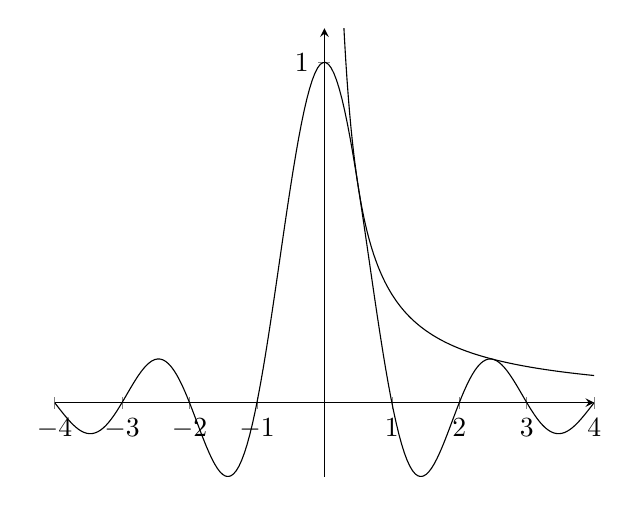
\begin{tikzpicture}
    \begin{axis}[
    axis lines = middle,
    ytick = {0,1},
    xtick = {-6,-5,...,6},
 %   xticklabels = {$-\pi$},
    ymax = 1.1,
    ]
      \addplot[domain=-4:4,samples=200]{sin(deg(pi*x))/(pi*x)};
      \addplot[domain=0.1:4,samples=200,black]{1/pi/x};
     % \addplot[domain=-6:6,samples=200]{-1/pi/x};
    \end{axis}
  \end{tikzpicture}
  \caption{Funzione sinc(x)}
\end{figure}
è un segnale di energia data la sua natura convergente all'infinito.

In questo caso i coefficienti $c_k$ corrispondono a punti sul grafico della
funzione sinc, nel punto $k=0$ si ottiene proprio il coefficiente $c_0$ pari
alla componente continua del segnale rappresentato mediante la serie di
Fourier, la componente continua è dunque pari ad $A\cdot D$ dunque il
\textit{duty cycle} esprime l'energia del segnale.

La funzione sinc ha dei
nulli in corrispondenza dei valori interi dell'argomento, ovvero sinc($x$) si
annulla nei multipli interi di $\pi$ dunque se $D = 0.5$ tutte le volte che $k$
è pari l'argomento del sinc è intero, dunque tutte le armoniche pari saranno
nulle.
Se invece il duty cycle è $D=1/3 = 0.\overline{3}$ tutte le armoniche
\textit{triple} ovvero multiple di 3 saranno nulle.

\section{Spettro di un segnale}
Con l'espansione in serie di un segnale, l'informazione ricavata è chiamata
solitamente \textbf{spettro}, si utilizza non solo per i segnali periodici ma
per una classe molto più ampia di segnali.
Lo spettro si compone di due diagrammi rappresentati da una coppia di sequenze :
\begin{itemize}
 \item Spettro di ampiezza $\{A_k\} $
 \item Spettro di fase $\{\phi_k\}$
\end{itemize}

Si possono riportare su uno \textit{Stem plot}, ovvero dei grafici a barre in
funzione della frequenza.
%Inserisci stem plot ampiezza e fase

Viene utilizzato il termine spettro perché queste due grandezze permettono di
classificare in maniera univoca i segnali.
